% !TeX spellcheck = en_GB
\documentclass[10pt,letterpaper,oneside]{article}
\usepackage{fontspec}
\usepackage{arev}
\usepackage[utf8]{inputenc}
\usepackage[T1]{fontenc}
\usepackage{amsmath}
\usepackage{amsfonts}
\usepackage{amssymb}
\usepackage{graphicx}
\usepackage{csquotes}
\usepackage{booktabs}
\usepackage{multicol}
\usepackage{enumerate}
\usepackage{microtype}
\usepackage[labelfont=bf,font={small}]{caption}
\usepackage{hyperref}
\usepackage{booktabs}
\usepackage{subcaption}
\usepackage{fancyhdr}
\usepackage{calc}
\usepackage[svgnames]{xcolor}
\usepackage{cleveref}

\newfontfamily\symbolfont{Symbola}
\usepackage[left=1in,right=1in,top=1in,bottom=1in,marginparwidth=0.25in]{geometry}

\usepackage[sorting=none]{biblatex}
\addbibresource{../bibliography.bib}

\author{Andreas Stöckel\\[0.5cm]Based on lecture notes by\\Chris Eliasmith and Terrence~C.~Stewart}

\fancyhf{}
\fancyhead[L]{SYDE 556/750 Lecture Notes}
\fancyhead[R]{Andreas Stöckel}
\fancyfoot[C]{\thepage}
\pagestyle{fancy}

\setlength{\parindent}{0em}
\setlength{\parskip}{0.5em}
\renewcommand{\baselinestretch}{1.25}
\renewcommand{\vec}[1]{{\mathbf{\mathrm{#1}}}}
\newcommand{\mat}[1]{{\mathbf{\mathrm{#1}}}}

\newcommand{\MakeTitle}[1]{
\maketitle
\begin{center}
	\includegraphics[width=0.5\textwidth]{../assets/uwlogo.pdf}\\[1cm]
	{#1}\
\end{center}

\vfill

\thispagestyle{empty}
\setcounter{page}{0}
\newpage

\pagenumbering{roman}
\tableofcontents
\newpage

\setcounter{page}{0}
\pagenumbering{arabic}}

\reversemarginpar

\newcommand{\ColorBox}[3]{{\par\hspace{0pt}\marginpar{\huge\raisebox{-1ex}{\symbolfont{#1}}}\ignorespaces\fboxsep=0.5cm\colorbox{#2}{\begin{minipage}[t]{\columnwidth-1cm}{#3}\end{minipage}}}}

\newcommand{\Note}[1]{\ColorBox{📌}{WhiteSmoke}{\textbf{Note:} #1}}
\newcommand{\Example}[1]{\ColorBox{💡}{WhiteSmoke}{\textbf{Example:} #1}}


\date{January 7, 2020}
\title{SYDE 556/750 \\ Simulating Neurobiological Systems \\ Lecture 1: Introduction}


\begin{document}

\MakeTitle{\textbf{Accompanying Readings: Chapter 1 of Neural Engineering}}

\section{Overview}

\Note{This entire lecture is meant to give you a broad, whirlwind overview of the material in the course. We are going to revisit most of the topics mentioned here in much more detail in the upcoming weeks.}

\subsection{Overall Goal of This Course}

The overall goal of this course is to explore methods for modelling and simulating large-scale neurobiological systems. By large-scale we mean that we are focusing on the properties of nervous \emph{systems} and less on the interaction between their individual components (i.e., individual neurons/synapses).

Put differently, our goal is to systematize the construction of brain models -- or at least the constructions of models of brain subsystems.

Beyond the fact that building brain models is the most interesting thing in the world\footnote{I will leave it up to the reader to decide whether this is a subjective statement.}, why should you be excited about this course? What are potential applications of the material we are going to discuss?
\begin{enumerate}[1.]
	\item \textbf{Figuring out how the brain works}
	\begin{itemize}
		\item Health applications (better treatment of diseases).
		\item Philosophical implications (new ways of understanding the mind and who we are).
	\end{itemize}
	\item \textbf{Building better AI systems}
	\begin{itemize}
		\item Understanding how the brain works may help us to build better AI systems.
		\item \enquote{Classical AI} (structured; symbolic) $\leftrightarrow$ \enquote{Deep Learning} (unstructured, \enquote{sub-symbolic}, \enquote{grounded}). We are discussing solutions that are somewhere in between, i.e., systems that are structured but still able to learn and use grounded symbols.
	\end{itemize}
	\item \textbf{Programming neuromorphic hardware}
	\begin{itemize}
		\item Neuromorphic hardware systems are inspired by brain-like information processing. The methods discussed in this course facilitate programming these systems~\cite{boahen2017neuromorph}.
	\end{itemize}
\end{enumerate}

\subsection{Theoretical Neuroscience and Levels of Organization}

\begin{figure}[t]
	\centering
	\includegraphics{media/levels.pdf}\\
	\caption{The scope of theoretical neuroscience and levels of organization.}
	\label{fig:levels}
\end{figure}

The approach we are taking with respect to building models of neurobiological systems can be broadly characterized as being under the umbrella of \emph{Theoretical Neuroscience}.

Nervous systems can be described at multiple levels of organization, each level catering to different kinds of questions. For example, analysing nervous systems at the level of individual neurons and synapses tends to answer questions about how computations are performed in a neural substrate. Questions about motor control and perception are better answered by looking at entire  networks (e.g.~the retinal microcircuits for vision, or the cerebellar microcircuit for motor control). Since each of these organizational levels is interesting on its own, there are entire subdisciplines of neuroscience that focus on a narrow range of levels~(\cref{fig:levels}).

When trying to answer broader questions, such as \enquote{How does the mind work?}, concerning oneself with just one level of organization is no longer sufficient. We need techniques that help us bridge multiple levels of organization. Furthermore, we need some way of quantifying the progress towards our goal, as well as systematic methods that reduce the overwhelming complexity we are facing.

The aim of Theoretical Neuroscience is to work towards these goals by generating compact models that summarize what has been learned in the individual subdisciplines and that foster communication between them \cite{abbott2001theoretical}.

To frame the idea of Theoretical Neuroscience more clearly, let us consider another field of science that has been working on a problem that is \emph{almost} as complex as trying to answer the question of \enquote{who we are}.

\subsection{Theoretical Neuroscience vs. Theoretical Physics: An Analogy}

\begin{table}[h]
	\centering
	\caption{Comparison between theoretical physics and theoretical neuroscience.}
	\begin{tabular}{p{4cm} p{4cm} p{4cm}}
		\toprule
								  &
								  \textbf{Theoretical\newline physics} & \textbf{Theoretical\newline neuroscience} \\
		\midrule
		\raggedleft\emph{Quantify} phenomena & $\vec{F} = m \vec{a}$ & $\hat{\vec x} = \mat D \vec a$ \\
		\midrule
		\raggedleft \emph{Summarize} lots of data & motion of objects & neural representation of information \\
		\midrule
		\raggedleft Speculative (generate hypotheses) & true for all velocities & true for all stimuli \\
		\bottomrule
	\end{tabular}
	\label{tbl:physics_vs_theoretical_neuroscience}
\end{table}

Theoretical Neuroscience as a field can perhaps be best described by comparing it to Theoretical Physics, which is concerned with the nature of reality, or, phrased as a question, attempts to understand \enquote{What exists?}. Just as in neuroscience, physics is divided into numerous sub-fields, with particle physics at the smallest and astrophysics at the largest scale. The goal of theoretical physics is to find overarching descriptions that apply to all sub-fields -- examples being conservation of energy, or (as an example of a useful, but clearly limited model) Newtons laws of motion (\cref{tbl:physics_vs_theoretical_neuroscience}). Both apply to celestial objects and everyday objects alike, i.e., span multiple levels of scale and organization.

To summarize, both fields are similar in that they attempt to find quantifications that summarize large corpora of data across vastly different scales using similar mathematical methods. The main difference lies in the question that is being answered (\enquote{What exists?} vs. \enquote{Who are we?}). Furthermore, since biology tends to be highly nonlinear, limiting the potential of mathematical analysis, Theoretical Neuroscience has to rely on even more numerical simulations than Theoretical Physics.

\section{Neural Modelling}

To make sure that a theory from Theoretical Neuroscience, or, more broadly, \emph{any} theory about cognition, is useful, we should be able to use it to build models that make predictions about cognitive systems.

\Note{Note that this implies that our theories (or \enquote{frameworks}) must be precise enough to be turned into a mathematical model -- for example, many theories from Psychology do \emph{not} pass this requirement.

Since our models will get complex quite quickly, we must most certainly use some kind of computer simulation. Correspondingly, Theoretical and Computational Neuroscience are often quite closely related.}

In general, researchers often distinguish between the following kinds of models:
\begin{itemize}
	\item \textbf{Single neuron models}\\
	May include spikes, spatial structure, various ion channels, etc.
	\item \textbf{Small network models}\\
	May either use spiking neurons, rate neurons, mean fields, etc.
	\item \textbf{Large network/cognitive models}\\
	May either use biophysics, pure computation, anatomy, etc.
\end{itemize}
Ideally, we would like to have a framework that allows us to include levels of detail below any higher level as desired. Of course, the \enquote{correct} highest level depends on the question that is being asked. Our goal in this course is to be able to build models that elicit some kind of high-level behaviour, or \emph{function} -- either through motor control, or by solving cognitive tasks. We will refer to this kind of model as a \enquote{functional model}. As a consequence, we focus less on single neuron and small network models on their own, since these are often not sufficient to produce the functions we are interested in.

\Note{The term \emph{functional model} may be a little unfortunate since \emph{functional} is quite overloaded. As described above, we use \emph{functional} solely in the sense of \enquote{producing a behaviour} or \enquote{solving a cognitive task}.}

\subsection{Problems with current modelling approaches}

Classically, there have been two different approaches for constructing the kind behavioural models we are interested in: \enquote{bottom-up}, large-scale neural models and \enquote{top-down} cognitive models. Both approaches have various problems that -- in our opinion -- disqualify them from being useful theories in the \enquote{Theoretical Neuroscience} sense defined above.

\Note{We are \emph{not} saying that the approaches described below are useless! As with any scientific project, \enquote{usefulness} depends on the question that is being asked. In the context of this course, we are trying to build \enquote{functional models} (in the sense defined above), and the problems discussed below are solely with respect to this goal.}

\paragraph{Bottom-up, large-scale neural models}
Examples of this kind of approach would be (parts of) the Human Brain Project (HBP; \cite{markram2012human}) or the \href{https://www.darpa.mil/program/systems-of-neuromorphic-adaptive-plastic-scalable-electronics}{DARPA SyNAPSE} research program \cite{morgan2011darpa,merolla2014million}. Here, the general idea seems to be to collect as much information as possible about \enquote{canonical microcircuits} and to simulate these in large scale on either supercomputers or specialised neuromorphic hardware (see \cite{komer2016unified} for a more thorough discussion of the HBP).

The idea of canonical microcircuits may be attractive from a theoretical perspective. However, this seems to ignore that the brain consists of highly specialised structures. As we will discuss next, different parts of the brain are very dissimilar in terms of connectivity, cell types, as well as the type of input and output.

Furthermore, it is unclear how these projects hope to produce higher level behaviour beyond matching low-level neurophysiological data. Surely, intelligent behaviour does not just \enquote{emerge} by blindly repeating the same circuits over and over again.

\paragraph{Top-down cognitve models}
Top-down approaches can be characterized by foremost focusing on the behaviour and to a much lesser degree on the implementation of the behaviour in a neural substrate. This kind of approach is often taken in Cognitive Science and (if a computational model is provided) in Psychology. A variety of modelling frameworks exists that describe cognition in terms of simple computational building blocks that can be connected. Examples of modelling frameworks that follow this particular approach include \href{http://act-r.psy.cmu.edu/}{ACT-R} and \href{https://soar.eecs.umich.edu/}{Soar}.

The problem with these approaches is that the models constructed in these frameworks are disconnected from neuroscience, which makes it hard to make predictions about e.g.~neural activities or, on a higher level, reaction times and error rates.

Top-down modelling frameworks also have the problem of having no \enquote{bridging laws}. For example, if we were to build one part of our model in greater biological detail, it would be unclear how to build an interface between these levels of organization. One could argue that this is a bit like having rules of chemistry that never mention that \enquote{it's all built out of atoms and electrons}.

Because of these missing \enquote{bridging laws}, it is also not really practical to constrain the model according to data from neuroscience. For example, the mathematical equations that are being used to describe computation within the model are not constrained. However, as we will see in the upcoming weeks, a neural substrate may not be particularly good at computing certain functions.

As mentioned in the above note, these restrictions are surely fine for many research questions. One might (conversely) ask whether we actually understand the brain enough to provide \enquote{bridging laws} and to accurately constrain our models. The desire to provide a framework that links high-level behaviour down to neural activities may be met with the same scepticism as a computer science student who sets out to understand how a word processor works, but ends up worrying about transistors and solid-state physics.

\Note{One problem with this analogy is that in the case of computers we -- the scientific community -- understand all the laws that bridge between different levels of organization/abstraction. Trying to define similar laws for cognition is \emph{exactly} what we try to do in Theoretical Neuroscience.}

\Aside{For more fun but (perhaps flawed) analogies between neuroscience and computer science see \enquote{Could a Neuroscientist Understand a Microprocessor?} \cite{jonas2017could}.}


\subsection{The Brain}

We ended the last section asking whether we actually know enough about brains in order to expertly constrain our models and to define bridging laws. So, what \emph{do} we know about our brains?

Let's start with some basic facts about the human brain:\footnote{For those of you who still find this a little too abstract, take a look at this \YouTube[video showing an unfixed (i.e.,~untreated) human brain]{jHxyP-nUhUY} (warning: dead human body parts). In case you'd like to experience this in real life, take PSYCH~784.}
\begin{itemize}
	\item \textbf{Weight:} \SI{2}{\kilogram} (2\% of the body weight)
	\item \textbf{Power consumption:} \SI{20}{\watt} (25\% of the body's total power consumption)
	\item \textbf{Surface area:} \SIrange{1500}{2000}{\centi\metre\squared} (roughly four A4/letter pages of paper)
	\item \textbf{Number of neurons:} \SI{100} billion ($10^{11}$, \SI{150000}{\per\milli\metre\squared})
	\item \textbf{Number of synapses:} 100 trillion ($10^{14}$, about $1000$ per neuron)
\end{itemize}

\Note{If we were able to simulate 1000 neurons in realtime at about \SI{1}{\watt} (which is roughly the case for simple neuron models and specialised neuromorphic hardware, not counting any interconnect), a computer simulating the entire brain would consume about \SI{100}{\mega\watt}, i.e., the power output of an entire medium-scale power plant. That is almost 7 orders of magnitude more than what biology requires.}

\paragraph{Brain Structure}

\begin{figure}
	\centering%
	\begin{subfigure}{0.575\textwidth}%
		\centering%
		\includegraphics[height=8cm]{media/psm_v35_d759_diagram_of_the_left_cerebral_hemisphere.jpg}%
		\caption{Labelled lateral view of the left hemisphere}%
		\label{fig:brain_lateral}%
	\end{subfigure}%
	\begin{subfigure}{0.425\textwidth}%
		\centering%
		\includegraphics[height=8cm]{media/jean_baptiste_marc_bourgery_atlas_of_anatomy_human_brain.jpg}%
		\caption{Sagittal cross-section}
		\label{fig:brain_sagittal}
	\end{subfigure}%
	\caption{Illustrations depicting the human brain. \textbf{(a)} From \href{https://archive.org/details/popularsciencemo35newyuoft/page/n6}{\emph{Popular Science Monthly, Volume 35}} (1889) via \href{https://commons.wikimedia.org/wiki/File:PSM_V35_D759_Diagram_of_the_left_cerebral_hemisphere.jpg}{Wikimedia}. \textbf{(b)} Illustration by Jean-Baptiste Marc Bourgery, \emph{Traité complet de l'anatomie de l'homme} (1831 to 1854) via \href{https://commons.wikimedia.org/wiki/File:Human_brain.jpg}{Wikimedia}.}
\end{figure}

As can be seen in \cref{fig:brain_lateral,fig:brain_sagittal}, the human brain has several visually clearly distinct features. The most prominent of these structures is the Cerebral Cortex (the \enquote{folded} part at the top in \cref{fig:brain_sagittal}; each peak of a \enquote{fold} is called \emph{gyrus}, the corresponding trough is called \emph{sulcus}). Furthermore, we can clearly see the Cerebellum (the sponge-shaped \enquote{appendix} at the back of the brain), as well as the Brain Stem (the grey region extending into the spinal cord).

Cerebral cortex has historically been subdivided into different \enquote{lobes} (\cref{fig:brain_lateral}), particularly the \enquote{Frontal Lobe}, \enquote{Temporal Lobe} (temple $\hat=$ lateral/side), \enquote{Occipital Lobe} (occiput $\hat=$ lat.~back of the head), \enquote{Parietal Lobe} (paries $\hat=$ lat.~\enquote{wall}; top of the head). As it turns out, these subdivisions are not only purely anatomical, but also have functional significance.

Smaller features include the locus coeruleus, thalamus, amygdala, hypothalamus, substantia nigra, etc., which are not (well) visible in the illustrations here.

To summarize, the brain is highly structured, even at a macro-scale. We should take this structure into account when building cognitive models! Furthermore, there are many latin and greek names that you can remember (but don't feel obliged to) and impress your friends.

\Note{An introductory neuroscience book \cite{kandel2012principles} or a clinical neuroanatomy book (for example \cite{splittgerber2018snell}) may be good places to start in case you want to learn more about brain structure.}

\paragraph{Neurons and Synapses}

\begin{figure}
	\centering
	\begin{subfigure}[c]{0.56\textwidth}%
		\centering%
		\vspace{4.65201mm}%
		\includegraphics{media/neuron_sketch.pdf}%
		\vspace{4.65201mm}%
		\caption{Single neuron}%
		\label{fig:single_neuron}
	\end{subfigure}%
	\begin{subfigure}[c]{0.44\textwidth}%
		\centering%
		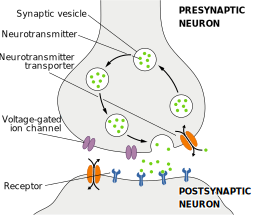
\includegraphics{media/synapse_schematic.pdf}%
		\caption{Chemical synapse}%
		\label{fig:chemical}
	\end{subfigure}
	\caption{Neurons and Synapses. \textbf{(a)} Sketch of a schematic biological model neuron. Input spikes arrive at synapses located at the dendrites and are processed in the cell body. Resulting output spikes travel along the axon to the axon terminals, where they connect to other neurons or a neuromuscular junction. From \cite{stoeckel2015design}~(fig.~2.3); inspired by \cite{kandel2012principles}~(fig.~2.2). \textbf{(b)} Diagram detailing synaptic transmission at a chemical synapse. From \cite{stoeckel2015design}~(fig.~2.10); adapted from \href{https://commons.wikimedia.org/wiki/File:SynapseSchematic_en.svg}{Wikimedia}.}
\end{figure}

The smallest unit of computation in the brain is usually assumed to be a single nerve cell, or \emph{neuron} (\cref{fig:single_neuron}). The interfaces between neurons are called synapses. Synapses are either \enquote{chemical} (\cref{fig:chemical}), or \enquote{electrical} (in some regions, e.g.,~retina).

In contrast to what the text-book illustration of \cref{fig:single_neuron} might suggest, neurons come in various visually distinct shapes and are often organised in a very chaotic fashion (cf.~panel \textbf{B}, \cref{fig:neuron_techniques}). Estimates of the number of neuron types range between 100 and 1000. Each neuron has beetween $1$-$200\,000$ inputs and outputs; the total axon length in the brain is estimated to be \SI{72}{\kilo\meter} (cf.~panels \textbf{D, E}, \cref{fig:neuron_techniques}).

Advances in scanning techniques allow researchers to reconstruct neural networks down to a nanometer scale, which means that we will have access to the \enquote{wiring diagram} of entire brain regions (see this \YouTube[National Geographics Video]{nvXuq9jRWKE} and this \YouTube[TEDx Talk]{F37kuXObIBU} by Jeff Lichtman).

\Aside{Scales of convergence and divergence. Granule cells in the cerebellum are one of the smallest neuron type in the brain. They receive input from exactly $4$-$5$ pre-synaptic neurons. Since more than half of all neurons in the brain are granule cells, the \emph{median} number of receiving synapses per neuron is $4$-$5$. Each Granule cell projects (diverges) onto $400$-$600$ Purkinje cells. Each Purkinje cell receives input from $175\,000$ granule cells.}

\begin{figure}
	\centering
	\includegraphics[width=\textwidth]{media/chédotal_richards_2010_techniques.png}
	\caption{Panels showing different techniques for labelling axon tracts and circuits in the mammalian brain. \textbf{A} Carbocyanine dye labeling of a developing embryonic mouse brain (day 17). \textbf{B} shows a so called \enquote{brainbow} image of a mouse brain in which individual neurons are coloured in different hues. \textbf{C} Diffusion-weighted magnetic resonance image. \textbf{D, E} Tractography images of high angular resolution imaging (HARDI/q-ball).  Image and captions from \cite{chedotal2010wiring} (fig.~7).}
	\label{fig:neuron_techniques}
\end{figure}

\newpage

\subsection{Kinds of Data From the Brain}

We now have a rough overview of the overall \emph{structure} of the nervous system, both on a macro- and micro-scale. Gathering this kind of structural data is the subject of neuroanatomy and cellular neuroscience, and of course, we should use these data -- for example macro- and micro-scale connectivity -- to constrain our models. But apart from these structural properties, what kind of empirical data from living brains do we have access to that can be used to either further constrain our model, or to test its predictions?

\subsubsection{Non-invasive}

\begin{figure}
	\begin{subfigure}[b]{0.33\textwidth}%
		\centering%
		\includegraphics[height=6.5cm]{media/kanwisher_et_al_1997_fusiform_fmri.png}%
		\caption{fMRI study}%
		\label{fig:fmri}
	\end{subfigure}%
	\begin{subfigure}[b]{0.3\textwidth}%
		\centering%
		\includegraphics[height=6.5cm]{media/eeg_recording_cap_small.jpg}%
		\caption{EEG cap}%
		\label{fig:eeg_cap}
	\end{subfigure}%
	\begin{subfigure}[b]{0.36\textwidth}%
		\centering%
		\includegraphics[height=6.5cm,trim=0 0 1cm 0,clip]{media/eeg_electroencephalogram.png}%
		\caption{Electroencephalogram}
		\label{fig:electroencephalogram}%
	\end{subfigure}
	\caption{Non-invasive brain data. \textbf{(a)} fMRI study of the \enquote{Fusiform Face Area} in the \enquote{Fusiform Gyrus} \cite{kanwisher1997fusiform} (fig.~3). \textbf{(b)} EEG cap (image from \href{https://commons.wikimedia.org/wiki/File:Three_quarter_view_of_EEG_subject.jpg}{Wikimedia}). \textbf{(c)} Electroencephalogram (image from \href{https://commons.wikimedia.org/wiki/File:Spike-waves.png}{Wikimedia})}
\end{figure}

\emph{Non-invasive} data sources allow us capture data from a nervous system \emph{in vivo}, without requiring direct access to the brain and without inflicting permanent damage to the subject. Correspondingly, we are (fortunately) mostly restricted to this kind of data when studying human brains.

\paragraph{fMRI}
\emph{Functional magnetic resonance imaging} is a measure of whole-brain activity based on \emph{changes} in blood flow. Often this is based on the so called blood-oxygen-level dependent (BOLD) contrast (\cref{fig:fmri}).  A catalogue of data can be found at \url{https://neurosynth.org/}.
\begin{multicols}{2}
	\begin{itemize}
		\item[\OPlus] Whole-brain, 3D reconstruction (individual activity voxels, volume elements)
		\item[\OMeh] Medium spatial resolution (millimeters)
	\end{itemize}
	~\vfill\columnbreak
	\begin{itemize}
		\item[\OMinus] Low temporal resolution (seconds)
		\item[\OMinus] Signal is hard to interpret (differences, indirect, i.e.,~does \emph{not} measure spiking)
		\item[\OMinus] Has to be averaged over multiple trials
	\end{itemize}
\end{multicols}

\paragraph{EEG}
\emph{Electroencephalography} measures the electric activity at the scalp using an array of electrodes (\cref{fig:eeg_cap,fig:electroencephalogram}). Being isolated from the brain through several layers of bone and tissue, this method can at most capture large-scale communication between areas.
\begin{multicols}{2}
	\begin{itemize}
		\item[\OPlus] High time resolution
		\item[\OMeh] Relatively cheap
		\item[\OMeh] Artefacts (eye movement, swallowing)
	\end{itemize}
	\columnbreak
	\begin{itemize}
		\item[\OMinus] Low spatial resolution
	\end{itemize}
\end{multicols}

\subsubsection{Invasive}

In contrast to non-invasive data sources, invasive data sources require direct access to the brain and may result in permanent damage.

\paragraph{Lesion Studies}
Here the question is what effect damaging a certain part of the brain has. This may either be part of an experiment (in animals) or the result of an accident/disease (in humans). For example,
lesion of the occipital cortex leads to \enquote{blindsight} (blindness where some visual information is still unconsciously present),
lesion of the inferior frontal gyrus results in loss of the ability to speak (Broca's area),
lesion of the posterior superior temporal gyrus results in loss of the ability to understand speech (Wernicke's area),
lesion of the fusiform gyrus prevents recognition of faces and other visually complex objects,
and lesion of the medial prefontal cortex may affect moral judgment (controversial; see: Phineas Gage).
\begin{multicols}{2}
	\begin{itemize}
		\item[\OPlus] Informative about the functional relevance of an area
	\end{itemize}
	\columnbreak
	\begin{itemize}
		\item[\OMinus] Often permanently damaging (though techniques for reversible lesions exist)
	\end{itemize}
\end{multicols}

\paragraph{Single cell recording}
Here, electrodes (one or many) are placed in the brain. The electrode might not neccessarily be placed right at (or in) a neuron, so it will pick up the \emph{local field potential} (LFP; a superposition of neural activity from multiple cells). It is common to amplify the recorded signal and to send it to a speaker, which makes spikes audible (\YouTube{KE952yueVLA}).
\begin{multicols}{2}
	\begin{itemize}
		\item[\OPlus] High temporal resolution (microseconds)
		\item[\OPlus] High specificity (single or few neurons)
	\end{itemize}
	\columnbreak
	\begin{itemize}
		\item[\OMinus] Limited to a few cells
		\item[\OMinus] Damaging over time
	\end{itemize}
\end{multicols}


\paragraph{Multi-electrode recordings}
Here a so called \enquote{tetrode} (an electrode with multiple tips) or a \enquote{Microelectrode Array} (MEA; \enquote{Utah Array}) is inserted into the brain (\YouTube{lfNVv0A8QvI}).
\begin{multicols}{2}
	\begin{itemize}
		\item[\OPlus] High temporal resolution (microseconds)
		\item[\OMeh] Up to $\approx$ 100 cells with one array
		\item[\OMeh] Requires post-processing (e.g.,~extraction of individual neurons from LFPs)
	\end{itemize}
	\columnbreak
	\begin{itemize}
		\item[\OMinus] Damaging over time
	\end{itemize}
\end{multicols}

\paragraph{Calcium Imaging}
Use fluorescent calcium indicator to indicate the presence of $\mathrm{Ca}^{2+}$ ions inside a neuron, which is an indicator for neuronal activity. Calcium indicators can either be chemical (i.e.~an externally added substance) or produced by the cell through genetic modification (\YouTube[Video: Fish Embryo]{DGBy-BGiZIM}, \YouTube[Video: Stalking Fish]{CpejbZ-XEyM}).
\begin{multicols}{2}
	\begin{itemize}
		\item[\OPlus] High temporal resolution (milliseconds)
		\item[\OPlus] High spatial resolution (individual cells)
	\end{itemize}
	\columnbreak
	\begin{itemize}
		\item[\OMinus] Local
		\item[\OMinus] Invasive
	\end{itemize}
\end{multicols}

\paragraph{Optogenetics}
Modify individual types of neurons genetically, so they can either be stimulated or inhibited through light (\YouTube{v7uRFVR9BPU}).
\begin{multicols}{2}
	\begin{itemize}
		\item[\OPlus] High temporal resolution (milliseconds)
		\item[\OPlus] Targets individual cell types
		\item[\OPlus] Can examine function of brain circuits
	\end{itemize}
	\columnbreak
	\begin{itemize}
		\item[\OMinus] Local
		\item[\OMinus] Invasive
	\end{itemize}
\end{multicols}

\subsection{Summary}

To summarize, we have access to a vast amount of data describing the brain at both the macro- and micro-scale, and both in terms of its anatomy (i.e.,~structure) and physiology (i.e.,~mechanisms within the living system).

Scientists have constructed neural models at the scale of single detailed individual neurons, as well as millions (\YouTube[HBP Video]{_UFOSHZ22q4}) and billions (\YouTube[SyNAPSE Video]{WmChhExovzY}) of neurons. Still, we don't have good theories that connect behaviour and cognition to low-level neural data. In the words of Churchland and Sejnowski (1994), neuroscience is \enquote{data-rich and theory-poor}. This is still true today.

\Note{Problematically, neuroscientists do not agree as for what the right level of detail of neural models is. When the SyNAPSE project led by IBM's Dharmendra S.~Modha announced the simulation of a \enquote{cat-scale} brain with 1 billion neurons in 2009, the founder of the Human Brain Project (HBP), Henry Markram, denounced the SyNAPSE project as a \enquote{hoax and PR stunt} and called for Modha to be \enquote{strung up by the toes} \cite{adee2009cat}. 
	
Markham's rage did not -- as one might expect -- stem from the fact that IBM's \enquote{cat brain} did not do what one would expect from a functional brain (controlling behaviour), but merely from the fact that IBM's neurons were \enquote{too simple} and therefore cannot possibly constitute a full brain model. Markham's HBP and its predecessor, the BlueBrain project, make use of physiologically and anatomically detailed neuron models that are statistically connected. Yet, as of 2020, the HBP has similarly not presented a \enquote{functional} brain model.

Of course, this leaves that question as for what the right level of detail is to be counted as a \enquote{brain model}. Perhaps we should, as we have discussed above, focus on what actually matters -- connecting neural models to high-level behaviour.}

\section{The Neural Engineering Framework and the Semantic Pointer Architecture}

Now that we have spent some time discussing other approaches aiming at large-scale modelling of neurobiological systems and pointed out their potential shortcomings, it is time to introduce the approach at neural modelling we are going to discuss in this course. In particular, we are going to have a look at two different modelling techniques: the \emph{Neural Engineering Framework}, and the \emph{Semantic Pointer Architecture}.

\subsection{Neural Engineering Framework}
The \emph{Neural Engineering Framework} (NEF) has been proposed by Eliasmith and Anderson in their book \enquote{Neural Engineering} in 2003 \cite{eliasmith2003neural}. We will spend the first half of this course on discussing the NEF.

The goal of the Neural Engineering framework is to treat the brain as a purely physical system and to use techniques form engineering -- such as control theory, information theory, and signal processing theory -- to aid a \emph{functional} understanding of the brain in theoretical neuroscience. After all, building physical systems that perform a certain function and -- to this end -- \emph{understanding} physical systems in terms of their potential function lies at the heart of engineering practice.\footnote{This is akin to Richard Feynman's famous chalkboard note \enquote{What I cannot create, I do not understand.} \cite{richard1988richard}} Of course, a major difference lies in the fundamental components usually employed by nature and, conversely, be engineers. Natural systems have evolved, and their individual parts, such as neurons, are thus inherently diverse and \enquote{messy}. Engineers on the other hand often rely on precisely manufactured parts. So when applying engineering methods to neural modelling, we somehow have to take this messiness into account. As we will see later, we can actually use the \enquote{messiness} of neural systems to our advantage when building models.

The Neural Engineering Framework provides a systematic way to translate a vector-valued dynamical system into a spiking neural network. In other words, the NEF can be thought of as a \emph{neural compiler}, that turns a mathematical description into a spiking neural network. Most importantly, this translation process can be informed by the vast corpus of neuroscientific data collected over the past decades. To put it differently: given a mathematical model, and a set of neurobiological constraints, including neural tuning, neuron count, connectivity, and time constants, we can create a neural network that fulfils these constraints and approximates the mathematical model.

\subsection{Semantic Pointer Architecture}
The second technique -- which we are going to discuss, among other topics, during the second half of the course -- is the \emph{Semantic Pointer Architecture} (SPA). The SPA is a mathematical tool for building models of high level cognition. It is based on what's commonly referred to as a \emph{Vector Symbolic Architecture} (VSA) and has been described in the book \emph{How to Build a Brain} by Eliasmith published in 2013 \cite{eliasmith2013how}.

VSAs provide a way to implement discrete symbolic architectures as they have been used in classical aritficial intelligence research (\enquote{Good Old Fashioned AI}; GOFAI) on top of continuous vector spaces. The SPA in particular describes how such \enquote{symbol vectors}, also called \enquote{semantic pointers}, can be generated from sensory input, combined -- or bound to -- other semantic pointers, and decompressed back into either the sensory or motor domain.

\subsection{The NEF and SPA as tools for hypothesis generation}
While the NEF and SPA are independent concepts, they together provide a powerful tool for scientific exploration in theoretical neuroscience and cognitive science. In particular, the NEF provides a way to represent vector spaces in a neural substrate, and, conversely, the SPA provides a way to implement a cognitive architecture on top of vector spaces. In a sense, the NEF describes the computational substrate, whereas the SPA can make use of -- but is not limited to -- this substrate. Looking back at \cref{fig:levels} we see that the NEF and SPA together model biological systems from synapses and neurons up to entire central nervous systems. So far, no other modelling approach can achieve this. We will have a look at some examples of models that have been built using these methods in \cref{sec:examples}.

Of course, merely using these techniques does not magically mean that the models we build are good models of human cognition. In fact, depending on the kind of question we are trying to answer, our models are most definitively wrong, but that is just the nature of models. The true strength of any modelling technique is in aiding \emph{hypothesis generation}.

For example, in the context of the NEF and the SPA, we might have an hypothesis as for how a certain cognitive task could be solved in terms of the SPA. We furthermore know from empirical research which brain regions in are involved in solving this task, and as such have data from neuroscience. We can now use this data as constraints when mapping the model onto the brain using the NEF. The resulting spiking neural network model can then be simulated and probed in various ways. This allows us \emph{(a)} to \emph{verify} our hypothesis by comparing high-level behaviour data (e.g.,~timings and error rates) between human/animal subjects and our model and \emph{(b)} to make \emph{predictions} about what we should be able to measure in the case of experiments that have not been performed on real subjects.

\subsection{The Nengo Simulator}
In the end, the NEF and the SPA are just mathematical concepts. In order to aid scientists in pursuing the kind of hypothesis-driven research outlined above, we need tools that facilitate the construction of such models. The \enquote{\texttt{nengo}} (originally short for \enquote{\emph{N}eural \emph{Eng}ineering \emph{O}bjects}) neural network simulation package is such a tool. It not only provides convenient interfaces for building NEF and SPA models (as well as other kinds of artificial neural networks), but can also execute the resulting model on a variety of hard- and software-backends such GPUs and analogue and digital neuromorphic hardware.

\texttt{nengo} was originally developed by members of the Computational Neuroscience Research Group (CNRG) at the University of Waterloo \cite{bekolay2014nengo}. It is now developed by a company called ABR (Applied Brain Research). \texttt{nengo} is available free-of-charge for non-commercial use. It can be found at \url{https://nengo.ai} and \url{https://github.com/nengo}.

\Note{As part of the assignments we are going to write our own software implementation of the NEF. Correspondingly, for the sake of learning the underlying theory, you cannot use \texttt{nengo} at first. However, you are asked to use \texttt{nengo} for the last assignment, and are free to use it for the final project. So it definitively doesn't hurt to have a look at it.}

\section{Representation, Transformation, and Dynamics}

The Neural Engineering Framework is based on three principles: Representation, Transformation, and Dynamics. We will have a closer look at each of these principles in upcoming lectures, but for now, let's quickly summarize what each of these principles is about.

\subsection{Representation}

In order to solve complex tasks, nervous systems must construct \emph{representations} of their environment. A reasonable definition of \emph{representation} would be to say that a neuron \emph{represents} some aspect of the environment, if this neuron is active (or conversely, exactly not active) whenever a certain stimulus is present. In other words, if there is a causal relationship between the stimulus and the neural activity. However, in general, the question of how exactly neurons represent information is still open.

In accordance with the above, we think of representations in the NEF as the mapping between a \emph{value} that is being processed in the network and the corresponding \emph{activity} of a \emph{group} of neurons. Mathematically speaking, the neural activity can be seen as a vector $\vec a(t)$ in a high-dimensional vector space, whereas the corresponding value $\vec x(t)$ may be a situated in a lower-dimensional vector space.

For this concept of representation to be useful, we need to define a way to \emph{decode} the represented value from the neural activity, and also a way to \emph{encode} a value as neural activites. The NEF defines the decoding process in terms of a linear decoder, and the encoding process in terms of a nonlinear encoding.

Note that we talked about representations in terms of the activity of a \emph{population} -- also referred to as an \emph{ensemble} -- of neurons, and not in terms of the activity of individual neurons. This is an important difference that separates the NEF from many \enquote{classical} modelling approaches in neuroscience. The NEF focuses on neuron populations as the smallest representational unit, and not individual neurons.

\newpage

\Example{Famous examples of neural representation are place- and grid-cells. Here neural activity is correlated with the animal being a certain location (place cells,~\cite{okeefe1978hippocampus}), or within a certain patch of a multi-scale hexagon grid (grid cells,~\cite{hafting2005microstructure}, see \cref{fig:hafting_et_al_2005_grid_cells}).  We are going to revisit grid cells when we talk about spatial semantic pointers. Another, more classical example is orientation tuning in primary visual cortex. Here, cells represent the orientation of line-shaped features in the visual field. See \cref{fig:eliasmith_et_al_2003_orientation_tuning}.}

\begin{figure}[t]%
	\begin{subfigure}[b]{0.5\columnwidth}%
		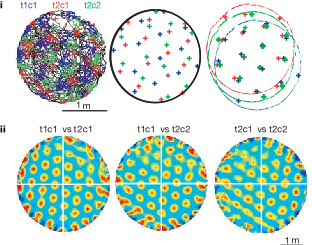
\includegraphics[width=\columnwidth]{media/hafting_et_al_2005_grid_cells.pdf}%
		\caption{Grid cells}%
		\label{fig:hafting_et_al_2005_grid_cells}%
	\end{subfigure}%
	\begin{subfigure}[b]{0.5\columnwidth}%
		\includegraphics[width=\columnwidth]{media/eliasmith_et_al_2003_orientation_tuning.pdf}%
		\caption{Visual orientation tuning}%
		\label{fig:eliasmith_et_al_2003_orientation_tuning}%
	\end{subfigure}%
	\caption{\textbf{Examples of neural representation.} \textbf{(a)} Grid cells. Top left: trajectory of the experimental animal while moving through space. Colours (ref, blue, green) correspond to the activity of three cells recorded from the dorsocaudal medial entorhinal cortex (dMEC). Top centre: peak activity locations for each cell. Top right: the individual cell peak activities are shifted to coincide with each other, highlighting the repeating structure in each cell. Bottom: cross-correlations between the individual cell activities. Figure copied from \cite{hafting2005microstructure}, fig.~3. \textbf{(b)} Example of visual orientation tuning of a cell in primary visual cortex of a macaque monkey. Figure copied from \cite{eliasmith2003neural}, fig.~3.1.}
\end{figure}

\Note{When talking about representations in this course, we generally refer to \enquote{transient} activities of the network, i.e.,~relatively short-lived signals. Of course, longer-lived states -- such as \emph{long-term memories} -- are also represented in the brain somehow, but we will talk about this separately when discussing learning.}

\Note{Having to think about representation in terms of vector spaces, may seem to be somewhat limiting. However, as we will see throughout the course, vectors are a very general mathematical construct that can be used to represent all kinds of things, including symbols, (bandlimited) functions over space and time, probability distributions, etc. If you'd like to, take a look at Chapter 3 in \cite{eliasmith2003neural}, which discusses function representation (we are most likely not going to discuss this particular chapter in detail; though we are going to discuss this concept in the context of representing functions over time).}

\subsection{Transformation}

Of course, merely being able to represent values within biologically plausible neural networks is not sufficient to explain complex behaviours. To this end, we need some notion of \emph{computation}, i.e., the ability to \emph{transform} a represented value $\vec x$ using a function $f(\vec x)$, and to store the resulting value $\vec y$ in another neural population.

In the NEF, we compute functions by choosing the \enquote{right} connection weights between two populations. In particular, since we have information about how the represented value $\vec x \in \mathbb{R}^m$ can be \emph{decoded} from, let's say, a source population $A$, and how values $\vec y \in \mathbb{R}^n$ are \emph{encoded} in a target population $B$, we can compute optimal connection weights ${\mat W}^f$ that realize a function $f : \mathbb{R}^m \rightarrow \mathbb{R}^n$.

\Note{The way in which we normally choose connection weights in the NEF is fundamentally different from popular approaches for training artificial neural networks, such as \emph{backpropagation}. Since we first think about what the individual neuron populations (comparable to a \enquote{layer} of neurons) \emph{represent}, we can optimally solve for connection weights on a connection-by-connection basis.
	
When \enquote{training} a network using back-propagation, the training procedure alters the connection weights across multiple layers simultaneously, hence changing what is being represented by individual neurons/populations of neurons. This makes back-propagation more powerful, since we don't have to know what the right representation and transformation is supposed to be. However, it also makes \enquote{training} inherently less interpretable, much slower, and less robust (with respect to hyperparameters). In other words, in the context of modelling neurobiological systems, there is no reason why we should use something such as backpropagation, as long as we have a good idea as for what the values being represented are, and which functions have to be computed to get from one representation to the next.

That being said, the NEF can be combined with backpropagation-like online-learning approaches in order to build systems that \emph{learn} over time. Again, we will talk about that during the second half of the course when we discuss learning.}

\subsection{Dynamics}

So far, the transformations we have talked process information in a \emph{feed-forward} fashion. However, most brain areas make heavy use of \emph{recurrent} (\enquote{backwards projecting}, or \enquote{cyclical}) connections. As it turns out, we can systematically use recurrent connections to implement arbitrary dynamical systems, i.e.,~equations of the form
\begin{align*}
	\frac{\mathrm{d}}{\mathrm{d}t} \vec x(t) = f(\vec x(t), \vec u(t)) \,,
\end{align*}
where $f : \mathbb{R}^m \times \mathbb{R}^n \rightarrow \mathbb{R}^m$ defines the differential equation, $\vec x$ is the current system state, and $\vec u$ is the input to the differential equation. Comparably to the feed-forward connections discussed above, we can easily find optimal recurrent connection weights ${\mat W}^f$ that approximate a certain dynamical system.

This is particularly useful for modelling phenomena such as (short-term) memory. For example, the following differential equation describing an \emph{integrator}
\begin{align*}
	\frac{\mathrm{d}}{\mathrm{d}t} \vec x(t) = \vec u(t) \,,
\end{align*}
can be used to \enquote{remember} an input $\vec u$ across time. Being able to implement dynamical systems allows us to incorporate approaches from control-theory into our models. This is helpful when trying to build motor control systems, but also for inference related tasks (cf.~\enquote{filters}, \enquote{observers} in control theory).

The ability to implement models with arbitrary dynamics is a central feature that sets the NEF apart from other modelling techniques. For example, the NEF provides a systematic approach for constructing stable attractor networks, which have been hypothesised to be an important building block of nervous systems for decades \cite{eliasmith2005unified}.

\Note{If time permits, we are going to discuss some newer, alternative approaches for building dynamical systems in a spiking neural substrate, such as the FORCE \cite{sussillo2009generating,nicola2017supervised} (an online dynamics learning approach) and EBN \cite{boerlin2011spikebased,boerlin2013predictive} (a method focused on efficient information transmission between neurons) at the very end of this term.}

\section{Examples}
\label{sec:examples}

As mentioned above, the NEF can be seen as a neural compiler. Given a quantitative description of a behaviour (e.g. an algorithm), we can solve for the connections between neurons that will approximate that behaviour. This works for a wide variety of neuron models, both detailed and simple neuron models (next lecture). In particular, as once would expect in real biological systems, the number of neurons affects the model's accuracy, while the neuron properties influence timing and computation. This means that we can make predictions about the behaviour of a system.

The following videos show some examples of the NEF and the SPA in action:
\begin{multicols}{2}
	\begin{itemize}
		\setlength{\itemsep}{0cm}
		\item \YouTube[Vision: character recognition]{2j9rRHChtXk}
		\item \YouTube[Vision: >1000 categories]{VWUhCzUDZ70}
		\item \YouTube[Problem solving: Tower of Hanoi]{sUvHCs5y0o8}
		\item \YouTube[Spaun: digit recognition]{f6Ul5TYK5-o}
		\item \YouTube[Spaun: copy drawing]{WNnMhF7rnYo}
		\item \YouTube[Spaun: addition by counting]{mP7DX6x9PX8}
		\item \YouTube[Spaun: pattern completion]{Q_LRvnwnYp8}
	\end{itemize}
\end{multicols}

\section{Conclusion}

To summarize, the approaches we are going to discuss in this lecture -- the Neural Engineering Framework (NEF) and Semantic Pointer Architecture (SPA) being among them -- allow us to model neurobiological systems at a scale unparalleled by competing approaches.

These techniques are particularly useful as a new way to test theories under neurological constraints, sometimes suggesting novel algorithms for solving problems in Artificial Intelligence (cf.~the examples above). Having a framework for scientific exploration of large-scale brain models facilitates gaining a better understanding of the brain, potentially leading to new medical applications, and an understanding of the mind and who we are.

\printbibliography

\end{document}